%%%%%%%%%%%%%%%%%%%%%%%%%%%%%%%%%%%%%%%%%
% Journal Article
% LaTeX Template
% Version 1.3 (9/9/13)
%
% This template has been downloaded from:
% http://www.LaTeXTemplates.com
%
% Original author:
% Frits Wenneker (http://www.howtotex.com)
%
% License:
% CC BY-NC-SA 3.0 (http://creativecommons.org/licenses/by-nc-sa/3.0/)
%
%%%%%%%%%%%%%%%%%%%%%%%%%%%%%%%%%%%%%%%%%

%----------------------------------------------------------------------------------------
%	PACKAGES AND OTHER DOCUMENT CONFIGURATIONS
%----------------------------------------------------------------------------------------

\documentclass[twoside]{article}

%\usepackage{lipsum} % Package to generate dummy text throughout this template

\usepackage[utf8]{inputenc} % acentos sin codigo
\usepackage[spanish, es-tabla]{babel} % espanol
\usepackage{graphicx} % graficos
\usepackage{longtable}
\usepackage{cleveref}
\usepackage[sc]{mathpazo} % Use the Palatino font
\usepackage[T1]{fontenc} % Use 8-bit encoding that has 256 glyphs
\linespread{1.05} % Line spacing - Palatino needs more space between lines
\usepackage{microtype} % Slightly tweak font spacing for aesthetics

\usepackage[hmarginratio=1:1,top=32mm,columnsep=20pt]{geometry} % Document margins
\usepackage{multicol} % Used for the two-column layout of the document
\usepackage[hang, small,labelfont=bf,up,textfont=it,up]{caption} % Custom captions under/above floats in tables or figures
\usepackage{booktabs} % Horizontal rules in tables
\usepackage{float} % Required for tables and figures in the multi-column environment - they need to be placed in specific locations with the [H] (e.g. \begin{table}[H])
%\usepackage{hyperref} % For hyperlinks in the PDF
\usepackage[colorlinks=true,linkcolor=blue]{hyperref}

\usepackage{lettrine} % The lettrine is the first enlarged letter at the beginning of the text
\usepackage{paralist} % Used for the compactitem environment which makes bullet points with less space between them

\usepackage{abstract} % Allows abstract customization
\renewcommand{\abstractnamefont}{\normalfont\bfseries} % Set the "Abstract" text to bold
\renewcommand{\abstracttextfont}{\normalfont\small\itshape} % Set the abstract itself to small italic text

\usepackage{titlesec} % Allows customization of titles
\renewcommand\thesection{\Roman{section}} % Roman numerals for the sections
\renewcommand\thesubsection{\Roman{subsection}} % Roman numerals for subsections
\titleformat{\section}[block]{\large\scshape\centering}{\thesection.}{1em}{} % Change the look of the section titles
\titleformat{\subsection}[block]{\large}{\thesubsection.}{1em}{} % Change the look of the section titles

\usepackage{fancyhdr} % Headers and footers
\pagestyle{fancy} % All pages have headers and footers
\fancyhead{} % Blank out the default header
\fancyfoot{} % Blank out the default footer
%\fancyhead[C]{Sistema Jigsaw Coding $\bullet$ \today $\bullet$ Vol. XXI, No. 1} %
\fancyhead[C]{Sistema Jigsaw Coding $\bullet$ \today $\bullet$ UNMSM} % Custom header text
\fancyfoot[RO,LE]{\thepage} % Custom footer text

\usepackage[apaciteclassic,nodoi]{apacite}

%\usepackage[round]{natbib}
\usepackage{multirow}
\usepackage{hhline}


\usepackage{listings}
\usepackage{color}

\lstset{ 
  basicstyle = \small,
  keywordstyle=\color{black}\bfseries,
  language=Java,
  frame=single,
  tabsize=3
}

%----------------------------------------------------------------------------------------
%	TITLE SECTION
%----------------------------------------------------------------------------------------

\title{\vspace{-15mm}\fontsize{24pt}{10pt}\selectfont\textbf{Sistema web para la enseñanza de algoritmos y programación usando Jigsaw}} % Article title

\author{
\large
\textsc{Leibnitz Rojas}\\[2mm] % Your name
\normalsize Univesidad Nacional Mayor de San Marcos \\ % Your institution
\normalsize \href{mailto:leiparov@gmail.com}{leiparov@gmail.com} % Your email address
\vspace{-5mm}
}
\date{}

%----------------------------------------------------------------------------------------

\begin{document}

\maketitle % Insert title

\thispagestyle{fancy} % All pages have headers and footers

%----------------------------------------------------------------------------------------
%	ABSTRACT
%----------------------------------------------------------------------------------------

\begin{abstract}

%\noindent \lipsum[1] % Dummy abstract text
Los estudios muestran que en muchas universidades del mundo, aún existen problemas cuando se trata de enseñar cursos relacionados a programación y algoritmos. Muchos estudiantes repiten las materias y otros simplemente abandonan en mitad de semestre. Por otro lado, existen muchas investigaciones respecto a cómo mejorar los problemas de aprendizaje de los estudiantes y no necesariamente en temas de programación. Muchos autores han aplicado diversas técnicas de aprendizaje colaborativo obteniendo resultados notables en sus alumnos. El objetivo del presente trabajo es desarrollar un sistema web para la enseñanza de algoritmos y programación a través de una técnica de aprendizaje colaborativo, el mismo que permitirá a los estudiantes desarrollar ejercicios y problemas de forma colaborativa.
\end{abstract}

%----------------------------------------------------------------------------------------
%	ARTICLE CONTENTS
%----------------------------------------------------------------------------------------

\begin{multicols}{2} % Two-column layout throughout the main article text

\section{Introducción}

A pesar de que la programación es el corazón de las ciencias de la computación, y por ende, la mayoría de las carreras de computación tienen cursos de programación, los resultados son desalentadores pues existen muchos estudios multi institucionales que indican que hay serias deficiencias en el aprendizaje de alumnos que han pasado uno o más cursos de programación \cite{mccracken_multi-national_2001,lister_multi-national_2004,Tenenberg_studentsdesigning_2005}. Algunas instituciones han logrado mejorar los cursos de programación adoptando el Python como primer lenguaje de programación. Así lo indica \citeA{nikula_python_2007}.\\

Según \citeA{knobelsdorf_teaching_2014}, los altos ratios de fracasos en los cursos de introducción a la teoría de las ciencias de la computación son un problema comun en las universidades de Alemania, Europa, y NorteAmérica, pues los alumnos tiene dificultades con lo contenidos que por naturaleza son abstractos y teóricos. \cite{knobelsdorf_teaching_2014} plantean en su investigación ciertas modificaciones a la pedagogía de un curso dictado en la Universidad de Postdam, Alemania, las mismas que fueron motivadas por un enfoque de aprendizaje cognitivo.\\

Existen diversas técnicas para desarrollar el aprendizaje colaborativo en un aula de clase y una de ellas, muy conocida, es la técnica de Jigsaw o técnica de Rompecabezas. Esta técnica fue creada en (1978) por Aronson et al. y actualmente es una de las más importantes para fomentar la cooperación y discusión entre miembros de una comunidad de aprendizaje y es usada frecuentemente en ambientes face-to-face y en situaciones de aprendizaje en línea \cite{blocher_increasing_2005}.\\

%Definicion del problema
Hoy en día, muchos estudiantes tienen dificultades para llevar con éxito los cursos de algoritmos y programación, problema que se evidencia en el porcentaje de alumnos que desaprueban los exámenes, que desaprueban el curso o que simplemente se retiran a mitad de ciclo.\\

%Justificacion
El problema descrito en el párrafo anterior se justifica con el hecho de que la alta tasa de fracaso de los estudiantes de programación ha sido durante muchos años un tema polémico para las instituciones de aprendizaje con reportes de ratios de fracasos alrededor de $26\%$ a $40\%$. \cite{sheard_our_1998,truong_web_2003,lang_seven_2007,han_enhancement_2010}.\\

Además, la últimas investigaciones sobre el problema reflejan que éste aún persiste. Los altos porcentajes de fracasos en cursos introductorios de programación son un problema común en universidades en Alemania, Europa, y Norte Ámérica, ya que los alumnos tiene problemas para entender los contenidos de tales cursos debido a su abstracción y naturaleza teórica \cite{knobelsdorf_teaching_2014}.\\

En lo que respecta al uso de técnicas de aprendizaje colaborativo tenemos que \citeA{martinez_cooperative_2011} presentaron el diseño, implementación y evaluación de una estrategia de enseñanza basada en aprendizaje colaborativo para introducir el tema de álgebra relacional en un curso de base de datos. La estrategia fue evaluada desde las perspectiva del alumno y del profesor, y se encontró que entre el $78\%$ y el $92\%$ de los estudiantes consideraron que el trabajo en grupo enriqueció su aprendizaje, dando soporte al uso del aprendizaje colaborativo; y recientemente, \citeA{cliburn_team-based_2014} desarrolló el curso de Estructura de Datos a través del aprendizaje basado en equipos y el aprendizaje tradicional con el fin de comparar resultados en las evaluaciones de los estudiantes, y, aunque no encontró diferencias significativas entre ambas secciones de alumnos, aún continúa usando el aprendizaje en equipos debido a la alta satisfacción que los alumnos muestran en comparación con el método de enseñanza tradicional.\\

%------------------------------------------------

\section{Estado del arte}

\subsection*{LearnCS}
\emph{LearnCS!} es un entorno de programación creado específicamente para el uso de estudiantes de primer año de la carrera de ciencias de la computación. Este programa elimina la necesidad de los alumnos de tener que preocuparse por un editor de texto, comandos linux y proceso de compilación. LearnCS! proveee un entorno web en el cual los alumno pueden escribir, ejecutar y depurar programas usando un interfaz familiar y amigable. El compilador de C embebido que posee el sistema permite al alumno ejecutar sus programas con simplemente hacer click en un botón y obtener los resultados de ejecución de su código fuente \cite{lipman_learncs_2014}.\\

LearnCS! fue creado para proporcionar un ambiente de aprendizaje para estudiantes de informática de primer año. Sus principales objetivos son proporcionar asistencia útil al alumno en la construcción de un modelo mental de la máquina nocional de C a través de la visualización detallada de la memoria de \emph{LearnCS!} y sus mensajes de error integrados en las instalaciones de depuración, y para proporcionar que producen consejos que son útiles para el principiante para localizar y corregir errores de sintaxis\cite{lipman_learncs_2014}.\\

\subsection*{Jigsaw}
Jigsaw es una técnica de aprendizaje colaborativo y recientemente ha sido aplicada por \citeA{Buhr2014429} a un grupo de estudiantes de medicina  de la Universidad de Duke tal y como se describe en el artículo \emph{``Using the Jigsaw Cooperative Learning Method to Teach Medical Students About Long Term and Postacute Care''}. En este estudio se desarrolló una experiencia colaborativa usando la técnica de Jigsaw para exponer a los estudiantes sobre el cuidado intensivo a largo plazo  (LTPAC - Long Term and Post Acute Care) y así lograr que ellos conozcan las herramientas y roles del personal involucrado en este tipo de cuidados de pacientes en un asilo de ancianos. Para alcanzar este objetivo, pequeños grupos de estudiantes de medicina realizaron entrevistas al personal de LTPAC sobre sus respectivos roles. Estos grupos posteriormente fueron reorganizados en nuevos grupos conteniendo un estudiante de cada grupo original más un moderador y cada estudiante en los nuevos grupos tuvo que explicar sobre el rol del profesional LTPAC al cual había entrevistado \cite{Buhr2014429}.\\

\subsection*{Ideone API - Sphere Engine}
Sphere Engine, antes conocida como Ideone API, permite a los usuarios ejecutar código en múltiples lenguajes de manera online. Ideone es un compilador y una herramienta de depuración que soporta más de 60 lenguajes de programación. Através de la API, los desarrolladores pueden crear sus propias aplicaciones con fines educativos, personales o de negocios. Sphere Engine es un servicio web el cual puede ser accedido a través de protocolo SOAP.\\

Esta API posee las siguientes funcionalidades:

\begin{enumerate}
	\item Permite subir código fuente y compartirlo con otros usuarios.
	\item Permite ejecutar el código fuente con una data inicial en el lado servidor y en más de 60 lenguajes de programación diferentes.
	\item Permite descargar los resultados obtenidos en la ejecución del código fuente(salida, errores, información de compilación, tiempo de ejecución, uso de memoria, etc).
\end{enumerate}
%------------------------------------------------

\section{Aporte práctico}
\subsection*{Sistema Jigsaw Coding}
El Sistema Jigsaw Coding tiene como característica principal el permitir a los usuarios de perfil alumno poder resolver problemas de programación que el docente asigne para la sesión jigsaw. Este requisito está descrito en el caso de uso \textbf{Resolver problema} que se presenta en la \autoref{fig:cus_resolver_problema}. 

\begin{figure}[H]
	\centering	
	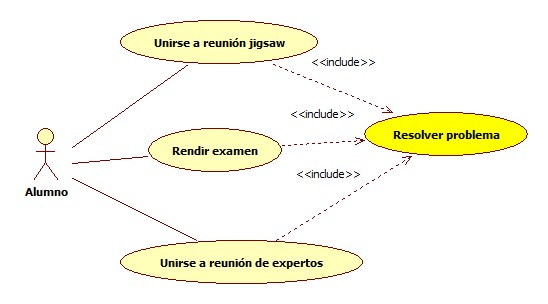
\includegraphics[scale=0.35]{figuras/casosdeuso/resolver_problema.jpg}
	\caption{Caso de uso Resolver problema}
	\label{fig:cus_resolver_problema}
\end{figure}

Como se observa en la \autoref{fig:cus_resolver_problema}, el caso de uso Resolver problema se encuentra como parte de los casos de uso Unirse a reunión de expertos, Unirse a reunión jigsaw y Rendir examen, y esto es porque, en cada una de las fases de la sesión jigsaw que se elabora en el sistema, se asignan problemas de algoritmos y programación que los alumnos deben desarrollar ya sea de manera grupal, o individual cuando se trata de un examen. El desarrollo de estos problemas se realiza en un editor de código fuente y luego se compila para obtener los resultados de la solución elaborada. 

\begin{figure}[H]
	\centering
	% Requires \usepackage{graphicx}
	\fbox{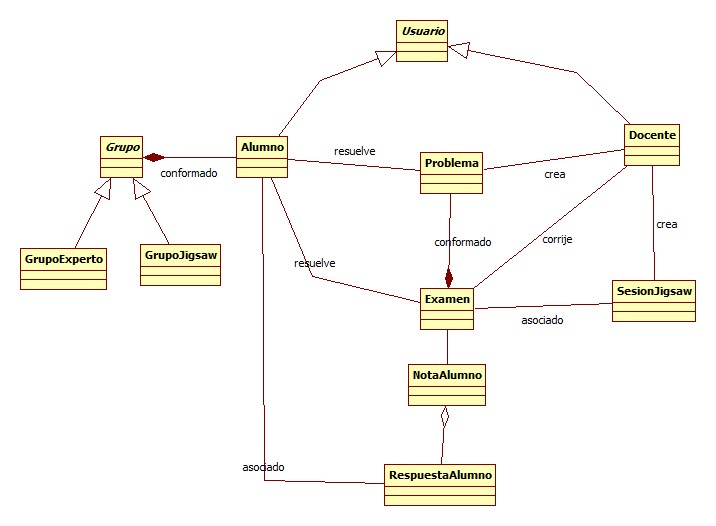
\includegraphics[scale=0.25]{figuras/sad/diagrama_de_clases.jpg}}\\
	\caption{Diagrama de Clases}\label{fig:c4_diagrama_de_clases}
\end{figure}

Por otro lado, tal como se muetra en el diagrama de clases de la \autoref{fig:c4_diagrama_de_clases}, el Sistema Jigsaw Coding permite el acceso a Usuario lo cuales pueden ser de dos tipos: Docente o Alumno. El docente puede crear problemas y además es el encargado de crear las sesiones jigsaw. El docente también es quien crea los examenes, los cuales están conformados por un conjunto de problemas y cada examen es resuelto por los alumnos, quienes para tal objetivo, deben resolver los problemas que componen cada examen. Por otro lado, los alumnos también resuelven problemas cada vez que se encuentran dentro de un grupo de expertos o un grupo jigsaw. Naturalmente, los examenes son evaluados por el docente y éste les asigna una nota a cada una de las respuestas que los alumnos envía al terminar su examen.\\

La vista de desarrollo muestra el sistema desde la perspectiva del programador y se ocupa de la gestión del software a implementar. Esto es, en esta vista se describe cómo estará dividido el sistema Jigsaw Coding en paquetes y las dependencias que hay entre ellos. Ver \autoref{fig:c4_diagrama_de_paquetes}.
\begin{figure}[H]
	\centering
	% Requires \usepackage{graphicx}
	\fbox{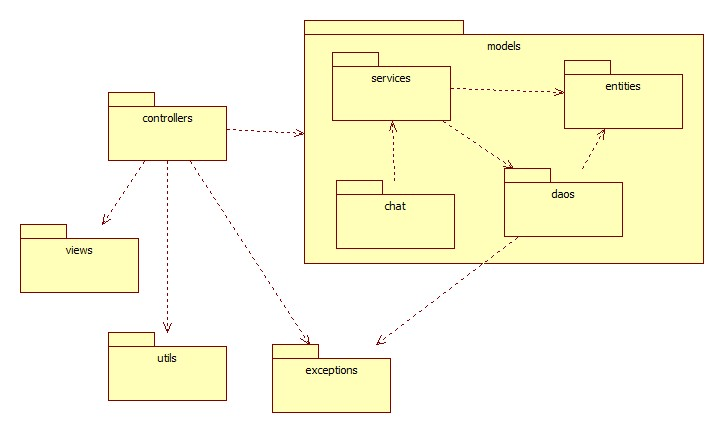
\includegraphics[scale=0.25]{figuras/sad/diagrama_de_paquetes.jpg}}\\
	\caption{Diagrama de Paquetes}\label{fig:c4_diagrama_de_paquetes}
\end{figure}
\begin{itemize}
	\item \textbf{controllers}\\Este paquete contiene todas las clases Controladores que sirven para gestionar el ruteo de páginas del sistema.
	\item \textbf{models}\\En este paquete se encuentran las clases de Servicios, Entidades y Acceso a Datos que son requeridas para el sistema.
	\item \textbf{views}\\Este paquete contiene todas las plantillas (\emph{*.scala.html}) que permitirán renderizar las páginas web del sistema.
\end{itemize}

Para la evaluación de la calidad del sistema se presentaron métricas de calidad basadas en la norma ISO-9126, la cual establece un estándar internacional para la evaluación de la calidad de los productos software \cite{iso9126-3}.

\begin{enumerate}
	\item Entendibilidad: ¿Qué porcentaje de los usuarios consideran que las funcionalidades del sistema son fáciles o muy fáciles de entender? \\ 
	\item Portabilidad: ¿En cuántos navegadores web puede usarse el sistema sin tener problemas?  \\ 
	\item Eficiencia: ¿Cuál es el promedio de tiempo de respuesta del Sistema Jigsaw Coding?\\
\end{enumerate}

	
%------------------------------------------------
\section{Caso de estudio}
El caso de estudio para la aplicación del Sistema Jigsaw Coding consta principalmente de estudiantes en cuyas carreras llevan o han llevado cursos relacionados a Programación y Algoritmos. \\

En esta ocasión, se tomará en cuenta a seis estudiantes a quienes se les hará partícipes de una sesión de clase jigsaw a través del sistema desarrollado en esta tesis.\\

En este caso de estudio se formarán 3 grupos expertos los cuales desarrollarán problemas de estructuras selectivas y repetitivas(\texttt{if - for - while}). De esa forma, cuando se llegue a la reunión jigsaw, los grupos jigsaw contarán con expertos en problemas sobre los 3 tipos de estructuras.\\

Para este caso de estudio se plante la resolución de los siguientes problemas de estructuras selectivas y estructuras repetitivas los cuales podrán ser desarrollados usando cualquiera de los 3 lenguajes que el Sistema Jigsaw Coding permite usar (Java, C++ o Python).\\

Para la fase de reunión de expertos y reunión jigsaw se usarán los siguientes problemas:

\begin{enumerate}
	\item \textbf{Par o impar}. Elaborar un programa que lea un entero y determine si es un número par o impar.
	\item \textbf{Múltiplos de 7}. Elaborar un programa que imprima los primeros 10 números múltiplos de 7 usando la estructura repetitiva \texttt{for}.
	\item \textbf{Números descendentes}. Elaborar un programa que imprima de forma descendente los primeros 20 numeros pares usando una estructura repetitiva \texttt{while}.
\end{enumerate}

Finalmente, para la fase de evaluación se combinará problemas de estructuras selectivas y repetitivas:

\begin{enumerate}
	\item \textbf{Número mayor}. Elaborar un programa que lea dos números enteros y muestre el número mayor.
	\item \textbf{n múltiplos de a}. Elaborar un programa que muestre los n primeros múltiplos de a, donde n y a son ingresados por teclado.
	\item \textbf{De número a texto}. Elaborar un programa que lea un número del 1 al 5 y lo muestre de forma escrita. Ejemplo 1 $\longrightarrow$ uno. Si es un número distinto a 1,2,3,4 o 5 que muestre el mensaje: Número equivocado.
	\item \textbf{Asteriscos}. Elaborar un programa que imprima la siguiente serie de asteriscos: \newline 	
	\hbox{*} \newline
	\hbox{**} \newline
	\hbox{***} \newline
	\hbox{****} \newline
	\hbox{*****} 	
\end{enumerate}
\section{Resultados}
Durante la fase de expertos se plantearon los problemas \emph{Múltiplos de 7, Par o impar, Números descendentes} y a continuación se presentan las soluciones de los alumnos.

\begin{center}
	GE\_DÁT\_ECM $\longrightarrow$ Múltiplos de 7.
\end{center}

Elaborar un programa que imprima los primeros 10 números múltiplos de 7 usando la estructura repetitiva \texttt{for}.

\lstset{language=C, breaklines=true, basicstyle=\footnotesize}
\begin{lstlisting}
# include <iostream>
using namespace std;
int main (){
int i;
cout<<"Los 10 primeros mutiplos de 7 son:"<<endl;
for(i=1;i<=10;i++){
cout<<i*7<<endl;
}
}
\end{lstlisting}
\begin{center}
	GE\_KMM\_DEG $\longrightarrow$ Par o impar.
\end{center}

Elaborar un programa que lea un entero y determine si es un número par o impar.

\lstset{language=Java, breaklines=true, basicstyle=\footnotesize}
\begin{lstlisting}
import java.util.Scanner;

class Ejercicio01 {
public static void main (String args[] ){
Scanner sc = new Scanner(System.in);

System.out.print("Introduzca un numero entero: ");
int n = sc.nextInt();

if(n%2==0) System.out.print("El numero es par");
else System.out.print("El numero es impar");
}
}
\end{lstlisting}

\begin{center}
	GE\_SMM\_MRB $\longrightarrow$ Números descendentes.
\end{center}

Elaborar un programa que imprima de forma descendente los primeros 20 numeros pares usando una estructura repetitiva \texttt{while}.

\lstset{language=C, breaklines=true, basicstyle=\footnotesize}
\begin{lstlisting}
#include <iostream>
using namespace std;
int main (){
int var = 40;
while(var > 1){
var = var - 2;
cout<<var<<endl;
}
return 0;
}
\end{lstlisting}

Cuando la fase de expertos finalizó, cada alumno fue reagrupado para dar inicio a la reunión jigsaw y en ella cada grupo resolvió los 3 problemas: \emph{Múltiplos de 7, Par o impar, Números descendentes}. \\

Por otro parte, luego de aplicar las métricas definidas para el sistema, se obtuvieron los siguientes resultados:

\begin{itemize}
	\item El Sistema es muy fácil de entender para el 66\% de los usuarios del caso de estudio.
	\item El Sistema es compatible y funciona correctamente en 4 navegadores web: Chrome, Internet Explorer, Ópera y Safari.
	\item El Sistema posee un tiempo promedio de respuesta de 1.3 segundos para las funcionalidades más importantes.
\end{itemize}

\section{Conclusiones}
\begin{itemize}
	\item Se desarrolló los antecedentes del problema y de la técnica. Así mismo, se planteó la justificación de y se definieron cuáles serían los objetivos y alcances de este trabajo de investigación.
	\item Se detalló algunos conceptos teóricos sobre aprendizaje colaborativo y cuáles son sus beneficios al aplicarlo en los estudiantes.
	\item Se plasmó el Estado del arte de las algunas herramientas y técnicas que permiten el aprendizaje colaborativo. 
	\item Se describió todo el desarrollo del Sistema Jigsaw Coding, para el cual se usó las mejores prácticas de RUP. Además, también se detalló el uso del sistema y se definieron 3 métricas de calidad que posteriormente serían aplicadas al sistema.
	\item Se presentó el caso de estudio sobre el cual se aplicaría el Sistema Jigsaw Coding. Se contó con las participación de 6 estudiantes universitarios y la sesión jigsaw comprendió temas de estructuras selectivas y repetitivas.
	\item Se aplicaron al Sistema Jigsaw Coding las métricas de calidad definidas y se presentaron los resultados obtenidos.
\end{itemize}

%----------------------------------------------------------------------------------------
%	REFERENCE LIST
%----------------------------------------------------------------------------------------
\bibliographystyle{apacite}
\bibliography{referencias}
%\begin{thebibliography}{99} % Bibliography - this is intentionally simple in this template
%
% 
%\end{thebibliography}

%----------------------------------------------------------------------------------------

\end{multicols}

\end{document}
